\chapter{Área de Estudo}
\label{cap:area_estudo}

A área de estudo compreende os estados de São Paulo (SP) e Rio Grande do Norte (RN), localizados, respectivamente, nas regiões Sudeste e Nordeste do Brasil (Figuras~\ref{fig:mapa_clima_sp} e~\ref{fig:mapa_clima_rn}). A seleção dessas unidades federativas fundamenta-se na representatividade de regimes climáticos distintos, evidenciada por diferenças fisiográficas e hidrológicas, bem como pela diversidade de tipos climáticos, biomas e padrões de uso e cobertura da terra. A caracterização climática regional é apresentada com base na classificação climática de Köppen-Geiger \citep{alvares2013}, enquanto os aspectos relacionados aos biomas e ao uso da terra seguem a classificação oficial dos biomas brasileiros e mapeamentos recentes de uso e cobertura da terra \citep{ibge_biomas2004,ibge_biomas_pagina,mapbiomas_collection8_platform}.

\section{Caracterização Climática}

\begin{figure}[h!]
\centering
\fbox{\includegraphics[width=0.7\textwidth]{mapa_clima_sp.png}}
\caption[Classificação climática de Köppen-Geiger no estado de São Paulo.]
{Distribuição espacial dos tipos climáticos segundo a classificação de Köppen-Geiger no estado de São Paulo. Predominam climas subtropicais úmidos, com variações associadas à sazonalidade da precipitação e à altitude, incluindo os tipos Cfa, Cwa e Cwb. Fonte: Alvares et al. (2013), adaptado.}
\label{fig:mapa_clima_sp}
\end{figure}

No estado de São Paulo (Figura~\ref{fig:mapa_clima_sp}), observa-se o predomínio de climas subtropicais úmidos, com variações espaciais associadas à altitude, à continentalidade e à proximidade com o oceano Atlântico. Na faixa litorânea, a atuação da Serra do Mar contrubio para maior precipitação orográfica e para a ocorrência de climas mais úmidos, enquanto regiões de maior altitude, como a Serra da Mantiqueira, apresentam temperaturas médias mais amenas. No interior do estado, predominam climas com estação seca mais bem definida no inverno.

\begin{figure}[h!]
\centering
\includegraphics[width=0.8\textwidth]{mapa_clima_rn.png}
\caption[Classificação climática de Köppen-Geiger no estado do Rio Grande do Norte.]
{Distribuição espacial dos tipos climáticos segundo a classificação de Köppen-Geiger no estado do Rio Grande do Norte. Observa-se o predomínio do clima semiárido quente (BSh), com diferenciação entre áreas com estação seca no inverno (BShw) e no verão (BSsh), abrangendo grande parte do interior do estado. Fonte: Silva (2009), adaptado.}
\label{fig:mapa_clima_rn}
\end{figure}

No Rio Grande do Norte (Figura~\ref{fig:mapa_clima_rn}), predominam condições climáticas semiáridas no interior do estado, caracterizadas por elevada irregularidade espacial e temporal da precipitação. Na faixa litorânea oriental e em áreas mais próximas ao oceano Atlântico, ocorrem climas tropicais mais úmidos, do tipo savana (Aw) e tropical chuvoso com estação seca curta (As). Essa configuração climática reflete a forte influência da Zona de Convergência Intertropical (ZCIT), cuja posição latitudinal controla a sazonalidade das chuvas na região.

\section{Localização Geográfica e Caracterização Fisiográfica}

O estado de São Paulo situa-se entre aproximadamente 19°S e 25°S de latitude e 44°W e 53°W de longitude, abrangendo uma área de cerca de 248.200 km$^2$. O relevo paulista é caracterizado pela predominância de planaltos e depressões, com destaque para o Planalto Atlântico, a Depressão Periférica Paulista e as faixas serranas da Serra do Mar e da Serra da Mantiqueira. Essas feições topográficas exercem influência direta sobre os padrões de circulação atmosférica regional, a distribuição da precipitação e os gradientes térmicos, especialmente em função dos efeitos orográficos e da proximidade com o Oceano Atlântico \citep{ibge_biomas_pagina}.

O clima predominante no estado é o subtropical úmido, com estação chuvosa bem definida durante a primavera e o verão austral, associada principalmente à atuação da Zona de Convergência do Atlântico Sul (ZCAS) e à passagem de sistemas frontais. A estação seca ocorre preferencialmente durante o inverno, quando a atuação de sistemas de alta pressão reduz a ocorrência de precipitação. A precipitação média anual apresenta elevada variabilidade espacial, com totais superiores a 1.600 mm em áreas serranas e litorâneas e valores inferiores a 1.200 mm em regiões do interior \citep{coelho2016}.

O estado do Rio Grande do Norte localiza-se entre aproximadamente 4°S e 7°S de latitude e 34°W e 38°W de longitude, com área aproximada de 52.800 km$^2$. O relevo é predominantemente plano a suavemente ondulado, com presença de planaltos residuais e depressões sertanejas, o que resulta em menor influência orográfica sobre a precipitação quando comparado ao Sudeste brasileiro \citep{ibge_biomas_pagina}.

O clima do Rio Grande do Norte varia do tropical úmido na faixa litorânea ao semiárido no interior do estado. A precipitação apresenta forte irregularidade espacial e temporal, com totais médios anuais superiores a 1.200 mm no litoral oriental e valores inferiores a 600 mm em extensas áreas do Sertão. A dinâmica climática regional é fortemente influenciada pela Zona de Convergência Intertropical (ZCIT), além de teleconexões oceânicas associadas às anomalias de temperatura da superfície do mar no Atlântico tropical \citep{marengo2017}.

\section{Biomas e Uso e Cobertura da Terra}

A caracterização dos biomas e das classes de uso e cobertura da terra neste estudo baseia-se nos dados do projeto MapBiomas \citep{mapbiomas_atbd_c8,souza2020_mapbiomas}, que fornece séries históricas anuais de uso e cobertura da terra para todo o território brasileiro a partir de imagens de sensoriamento remoto e algoritmos de classificação automatizada.

As classes de uso e cobertura da terra consideradas neste estudo seguem a legenda oficial do projeto MapBiomas (Coleção 9), contemplando formações naturais, áreas antrópicas e superfícies não vegetadas. A descrição dessas classes, bem como seus respectivos códigos, é apresentada na Tabela~\ref{tab:mapbiomas_classes}, permitindo a correta interpretação dos mapas temáticos apresentados a seguir.

\begin{table}[H]
\centering
\caption[Classes de uso e cobertura da terra do MapBiomas.]
{Descrição das classes de uso e cobertura da terra adotadas neste estudo, conforme a legenda oficial do projeto MapBiomas (Coleção 9). A coluna de cores corresponde à simbologia utilizada nos mapas temáticos apresentados.}
\label{tab:mapbiomas_classes}

\begin{minipage}{0.48\textwidth}
\centering
\begin{tabular}{c c l}
\hline
\textbf{Código} & \textbf{Cor} & \textbf{Classe} \\
\hline
3  & \cellcolor{green!60}  & Formação Florestal \\
4  & \cellcolor{green!40}  & Formação Savânica \\
5  & \cellcolor{green!80}  & Mangue \\
9  & \cellcolor{orange!70} & Formação Campestre \\
11 & \cellcolor{cyan!50}   & Campo Alagado e Á. Pantanosa \\
12 & \cellcolor{olive!60}  & Apicum \\
15 & \cellcolor{yellow!60} & Pastagem \\
20 & \cellcolor{pink!60}   & Cana \\
21 & \cellcolor{gray!40}   & Mosaico de Usos \\
23 & \cellcolor{orange!40} & Praia, Duna e Areal \\
24 & \cellcolor{red!40}    & Área Urbanizada \\
25 & \cellcolor{red!70}    & Outras Áreas não Vegetadas \\
29 & \cellcolor{brown!50}  & Afloramento Rochoso \\
\hline
\end{tabular}
\end{minipage}
\hfill
\begin{minipage}{0.48\textwidth}
\centering
\begin{tabular}{c c l}
\hline
\textbf{Código} & \textbf{Cor} & \textbf{Classe} \\
\hline

30 & \cellcolor{brown!80}  & Mineração \\
31 & \cellcolor{purple!50} & Aquicultura \\
32 & \cellcolor{olive!80}  & Sal \\
33 & \cellcolor{blue!60}   & Rio, Lago e Oceano \\
39 & \cellcolor{orange!80} & Soja \\
40 & \cellcolor{pink!40}   & Arroz \\
41 & \cellcolor{pink!20}   & Outras Lavouras Temporárias \\
46 & \cellcolor{green!30}  & Café \\
47 & \cellcolor{yellow!40} & Citrus \\
48 & \cellcolor{purple!30} & Outras Lavouras Perenes \\
49 & \cellcolor{violet!50} & Floresta Plantada \\
50 & \cellcolor{violet!20} & Restinga Arborizada \\
75 & \cellcolor{gray!20}   & Desconhecido \\
\hline
\end{tabular}
\end{minipage}

\end{table}

No estado de São Paulo, o bioma predominante é a Mata Atlântica, originalmente caracterizada por florestas densas e elevada biodiversidade \citep{ribeiro2009_atlanticforest}. Entretanto, a cobertura florestal remanescente encontra-se altamente fragmentada em decorrência de séculos de ocupação antrópica, restando atualmente uma fração reduzida da vegetação original \citep{sos_inpe_atlas}. O uso da terra no estado é dominado por atividades agropecuárias, especialmente agricultura mecanizada e pastagens, além de extensas áreas urbanizadas concentradas na Região Metropolitana de São Paulo e em polos industriais do interior.

\begin{figure}[H]
\centering
\fbox{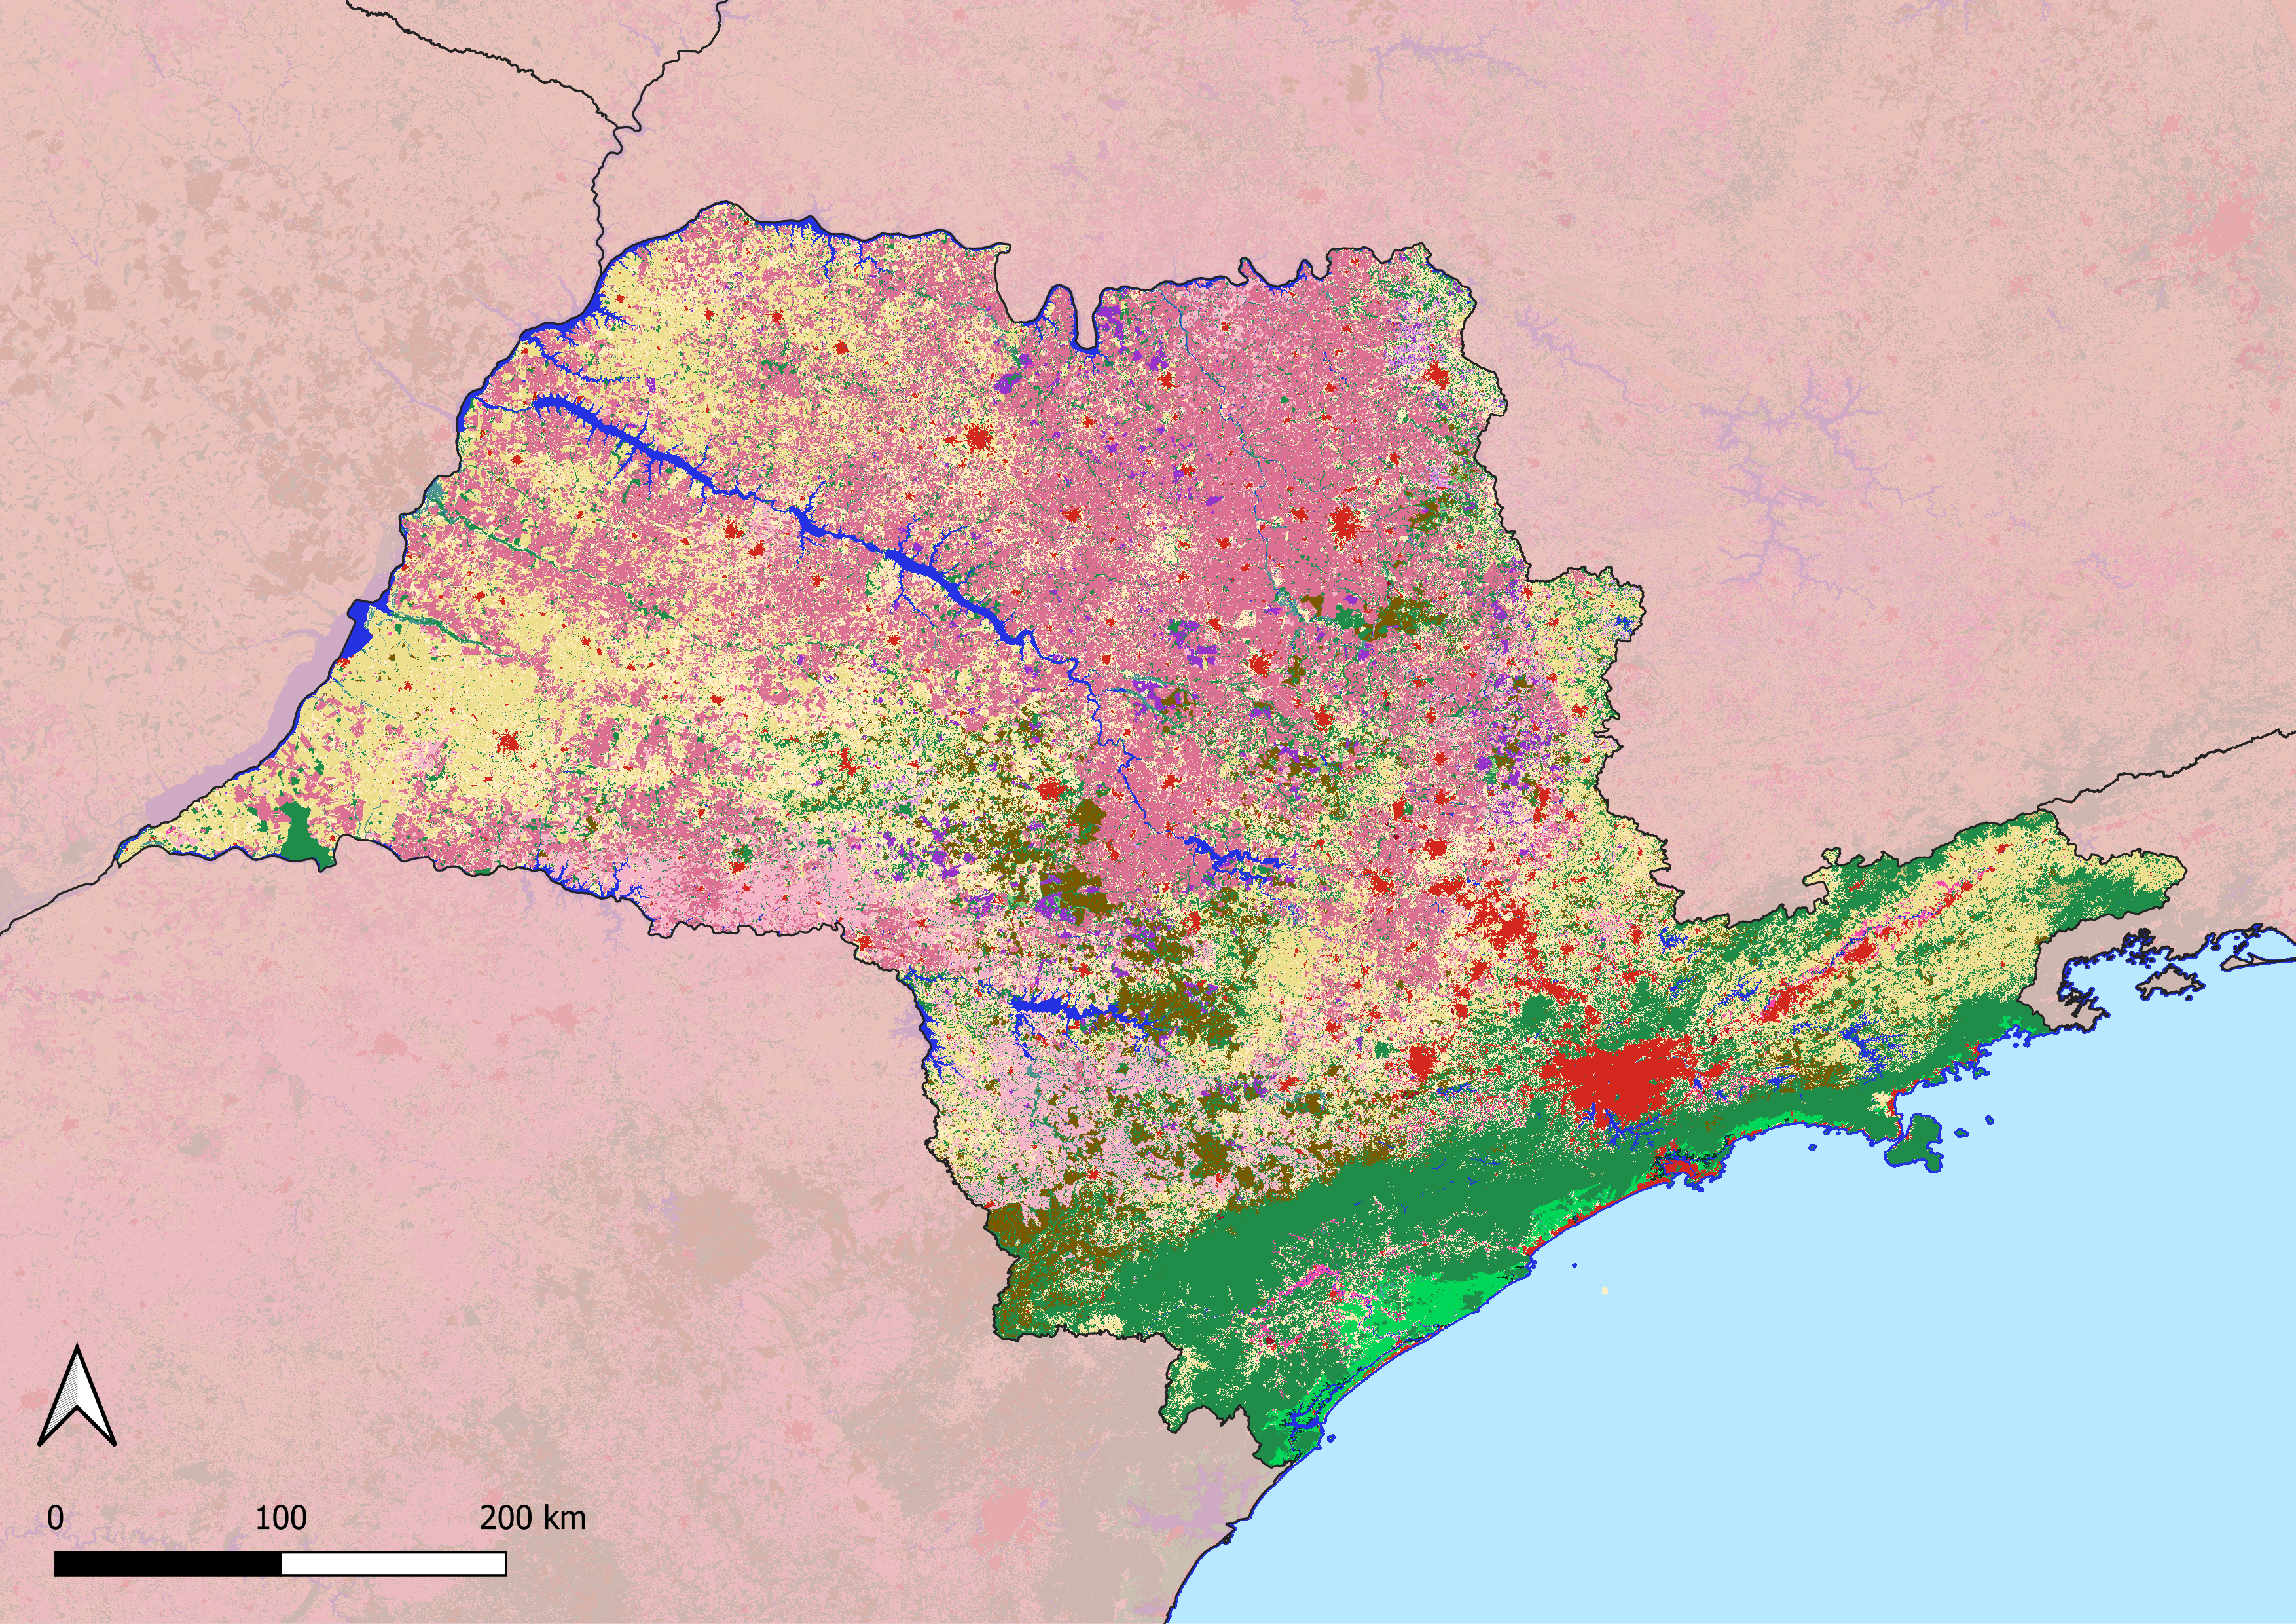
\includegraphics[width=0.9\textwidth]{tex/mapa_sp.png}}
\caption[Uso e cobertura da terra no estado de São Paulo.]
{Mapa de uso e cobertura da terra do estado de São Paulo, elaborado a partir da Coleção 9 do projeto MapBiomas (ano-base 2024). Fonte: Autor com auxílio do complemento MapBiomas Collection Official via QGIS.}
\label{fig:mapa_uso_sp}
\end{figure}

Com base na Figura~\ref{fig:mapa_uso_sp}, observa-se o predomínio de usos antrópicos no interior do estado, com destaque para as classes Pastagem, Cana e Mosaico de Usos (Tabela~\ref{tab:mapbiomas_classes}), associadas principalmente à atividade agropecuária. Os remanescentes de vegetação nativa concentram-se majoritariamente na faixa litorânea e em áreas serranas.

No estado do Rio Grande do Norte, o bioma Caatinga predomina na maior parte do território estadual, caracterizando-se por vegetação adaptada a condições semiáridas, elevada sazonalidade fenológica e forte dependência do regime de chuvas \citep{leal2003_caatinga}. Na faixa litorânea oriental, ocorre o bioma Mata Atlântica, associado a ambientes de maior umidade e à presença de ecossistemas costeiros, como manguezais e restingas \citep{ibge_biomas2004}. Assim como observado em São Paulo, o estado apresenta alterações significativas na cobertura vegetal natural decorrentes da expansão agropecuária, da urbanização costeira e da exploração de recursos naturais.

\begin{figure}[H]
\centering
\fbox{\includegraphics[width=0.9\textwidth]{tex/mapa_rn.png}}
\caption[Uso e cobertura da terra no estado do Rio Grande do Norte.]
{Mapa de uso e cobertura da terra do estado do Rio Grande do Norte, elaborado a partir da Coleção 9 do projeto MapBiomas (ano-base 2024). Fonte: Autor com auxílio do complemento MapBiomas Collection Official via QGIS.}
\label{fig:mapa_uso_rn}
\end{figure}

De acordo com a Figura~\ref{fig:mapa_uso_rn}, observa-se o predomínio de formações naturais associadas ao bioma Caatinga no interior do estado, intercaladas por áreas de uso agropecuário extensivo, principalmente Pastagem e Mosaico de Usos (Tabela~\ref{tab:mapbiomas_classes}). Na faixa litorânea, destacam-se áreas urbanizadas, remanescentes de Mata Atlântica e ecossistemas costeiros, refletindo condições climáticas mais úmidas e maior pressão antrópica.